%% template.tex
%% from
%% bare_conf.tex
%% V1.4b
%% 2015/08/26
%% by Michael Shell
%% See:
%% http://www.michaelshell.org/
%% for current contact information.
%%
%% This is a skeleton file demonstrating the use of IEEEtran.cls
%% (requires IEEEtran.cls version 1.8b or later) with an IEEE
%% conference paper.
%%
%% Support sites:
%% http://www.michaelshell.org/tex/ieeetran/
%% http://www.ctan.org/pkg/ieeetran
%% and
%% http://www.ieee.org/

%%*************************************************************************
%% Legal Notice:
%% This code is offered as-is without any warranty either expressed or
%% implied; without even the implied warranty of MERCHANTABILITY or
%% FITNESS FOR A PARTICULAR PURPOSE!
%% User assumes all risk.
%% In no event shall the IEEE or any contributor to this code be liable for
%% any damages or losses, including, but not limited to, incidental,
%% consequential, or any other damages, resulting from the use or misuse
%% of any information contained here.
%%
%% All comments are the opinions of their respective authors and are not
%% necessarily endorsed by the IEEE.
%%
%% This work is distributed under the LaTeX Project Public License (LPPL)
%% ( http://www.latex-project.org/ ) version 1.3, and may be freely used,
%% distributed and modified. A copy of the LPPL, version 1.3, is included
%% in the base LaTeX documentation of all distributions of LaTeX released
%% 2003/12/01 or later.
%% Retain all contribution notices and credits.
%% ** Modified files should be clearly indicated as such, including  **
%% ** renaming them and changing author support contact information. **
%%*************************************************************************


% *** Authors should verify (and, if needed, correct) their LaTeX system  ***
% *** with the testflow diagnostic prior to trusting their LaTeX platform ***
% *** with production work. The IEEE's font choices and paper sizes can   ***
% *** trigger bugs that do not appear when using other class files.       ***                          ***
% The testflow support page is at:
% http://www.michaelshell.org/tex/testflow/

\documentclass[conference]{IEEEtran}
% Some Computer Society conferences also require the compsoc mode option,
% but others use the standard conference format.
%
% If IEEEtran.cls has not been installed into the LaTeX system files,
% manually specify the path to it like:
% \documentclass[conference]{../sty/IEEEtran}





% Some very useful LaTeX packages include:
% (uncomment the ones you want to load)


% *** MISC UTILITY PACKAGES ***
%
%\usepackage{ifpdf}
% Heiko Oberdiek's ifpdf.sty is very useful if you need conditional
% compilation based on whether the output is pdf or dvi.
% usage:
% \ifpdf
%   % pdf code
% \else
%   % dvi code
% \fi
% The latest version of ifpdf.sty can be obtained from:
% http://www.ctan.org/pkg/ifpdf
% Also, note that IEEEtran.cls V1.7 and later provides a builtin
% \ifCLASSINFOpdf conditional that works the same way.
% When switching from latex to pdflatex and vice-versa, the compiler may
% have to be run twice to clear warning/error messages.






% *** CITATION PACKAGES ***
%
\usepackage{cite}
% cite.sty was written by Donald Arseneau
% V1.6 and later of IEEEtran pre-defines the format of the cite.sty package
% \cite{} output to follow that of the IEEE. Loading the cite package will
% result in citation numbers being automatically sorted and properly
% "compressed/ranged". e.g., [1], [9], [2], [7], [5], [6] without using
% cite.sty will become [1], [2], [5]--[7], [9] using cite.sty. cite.sty's
% \cite will automatically add leading space, if needed. Use cite.sty's
% noadjust option (cite.sty V3.8 and later) if you want to turn this off
% such as if a citation ever needs to be enclosed in parenthesis.
% cite.sty is already installed on most LaTeX systems. Be sure and use
% version 5.0 (2009-03-20) and later if using hyperref.sty.
% The latest version can be obtained at:
% http://www.ctan.org/pkg/cite
% The documentation is contained in the cite.sty file itself.






% *** GRAPHICS RELATED PACKAGES ***
%
\ifCLASSINFOpdf
  % \usepackage[pdftex]{graphicx}
  % declare the path(s) where your graphic files are
  % \graphicspath{{../pdf/}{../jpeg/}}
  % and their extensions so you won't have to specify these with
  % every instance of \includegraphics
  % \DeclareGraphicsExtensions{.pdf,.jpeg,.png}
\else
  % or other class option (dvipsone, dvipdf, if not using dvips). graphicx
  % will default to the driver specified in the system graphics.cfg if no
  % driver is specified.
  % \usepackage[dvips]{graphicx}
  % declare the path(s) where your graphic files are
  % \graphicspath{{../eps/}}
  % and their extensions so you won't have to specify these with
  % every instance of \includegraphics
  % \DeclareGraphicsExtensions{.eps}
\fi
% graphicx was written by David Carlisle and Sebastian Rahtz. It is
% required if you want graphics, photos, etc. graphicx.sty is already
% installed on most LaTeX systems. The latest version and documentation
% can be obtained at:
% http://www.ctan.org/pkg/graphicx
% Another good source of documentation is "Using Imported Graphics in
% LaTeX2e" by Keith Reckdahl which can be found at:
% http://www.ctan.org/pkg/epslatex
%
% latex, and pdflatex in dvi mode, support graphics in encapsulated
% postscript (.eps) format. pdflatex in pdf mode supports graphics
% in .pdf, .jpeg, .png and .mps (metapost) formats. Users should ensure
% that all non-photo figures use a vector format (.eps, .pdf, .mps) and
% not a bitmapped formats (.jpeg, .png). The IEEE frowns on bitmapped formats
% which can result in "jaggedy"/blurry rendering of lines and letters as
% well as large increases in file sizes.
%
% You can find documentation about the pdfTeX application at:
% http://www.tug.org/applications/pdftex





% *** MATH PACKAGES ***
%
%\usepackage{amsmath}
% A popular package from the American Mathematical Society that provides
% many useful and powerful commands for dealing with mathematics.
%
% Note that the amsmath package sets \interdisplaylinepenalty to 10000
% thus preventing page breaks from occurring within multiline equations. Use:
%\interdisplaylinepenalty=2500
% after loading amsmath to restore such page breaks as IEEEtran.cls normally
% does. amsmath.sty is already installed on most LaTeX systems. The latest
% version and documentation can be obtained at:
% http://www.ctan.org/pkg/amsmath





% *** SPECIALIZED LIST PACKAGES ***
%
%\usepackage{algorithmic}
% algorithmic.sty was written by Peter Williams and Rogerio Brito.
% This package provides an algorithmic environment fo describing algorithms.
% You can use the algorithmic environment in-text or within a figure
% environment to provide for a floating algorithm. Do NOT use the algorithm
% floating environment provided by algorithm.sty (by the same authors) or
% algorithm2e.sty (by Christophe Fiorio) as the IEEE does not use dedicated
% algorithm float types and packages that provide these will not provide
% correct IEEE style captions. The latest version and documentation of
% algorithmic.sty can be obtained at:
% http://www.ctan.org/pkg/algorithms
% Also of interest may be the (relatively newer and more customizable)
% algorithmicx.sty package by Szasz Janos:
% http://www.ctan.org/pkg/algorithmicx




% *** ALIGNMENT PACKAGES ***
%
%\usepackage{array}
% Frank Mittelbach's and David Carlisle's array.sty patches and improves
% the standard LaTeX2e array and tabular environments to provide better
% appearance and additional user controls. As the default LaTeX2e table
% generation code is lacking to the point of almost being broken with
% respect to the quality of the end results, all users are strongly
% advised to use an enhanced (at the very least that provided by array.sty)
% set of table tools. array.sty is already installed on most systems. The
% latest version and documentation can be obtained at:
% http://www.ctan.org/pkg/array


% IEEEtran contains the IEEEeqnarray family of commands that can be used to
% generate multiline equations as well as matrices, tables, etc., of high
% quality.




% *** SUBFIGURE PACKAGES ***
%\ifCLASSOPTIONcompsoc
%  \usepackage[caption=false,font=normalsize,labelfont=sf,textfont=sf]{subfig}
%\else
%  \usepackage[caption=false,font=footnotesize]{subfig}
%\fi
% subfig.sty, written by Steven Douglas Cochran, is the modern replacement
% for subfigure.sty, the latter of which is no longer maintained and is
% incompatible with some LaTeX packages including fixltx2e. However,
% subfig.sty requires and automatically loads Axel Sommerfeldt's caption.sty
% which will override IEEEtran.cls' handling of captions and this will result
% in non-IEEE style figure/table captions. To prevent this problem, be sure
% and invoke subfig.sty's "caption=false" package option (available since
% subfig.sty version 1.3, 2005/06/28) as this is will preserve IEEEtran.cls
% handling of captions.
% Note that the Computer Society format requires a larger sans serif font
% than the serif footnote size font used in traditional IEEE formatting
% and thus the need to invoke different subfig.sty package options depending
% on whether compsoc mode has been enabled.
%
% The latest version and documentation of subfig.sty can be obtained at:
% http://www.ctan.org/pkg/subfig




% *** FLOAT PACKAGES ***
%

%\usepackage{fixltx2e}
% fixltx2e, the successor to the earlier fix2col.sty, was written by
% Frank Mittelbach and David Carlisle. This package corrects a few problems
% in the LaTeX2e kernel, the most notable of which is that in current
% LaTeX2e releases, the ordering of single and double column floats is not
% guaranteed to be preserved. Thus, an unpatched LaTeX2e can allow a
% single column figure to be placed prior to an earlier double column
% figure.
% Be aware that LaTeX2e kernels dated 2015 and later have fixltx2e.sty's
% corrections already built into the system in which case a warning will
% be issued if an attempt is made to load fixltx2e.sty as it is no longer
% needed.
% The latest version and documentation can be found at:
% http://www.ctan.org/pkg/fixltx2e


%\usepackage{stfloats}
% stfloats.sty was written by Sigitas Tolusis. This package gives LaTeX2e
% the ability to do double column floats at the bottom of the page as well
% as the top. (e.g., "\begin{figure*}[!b]" is not normally possible in
% LaTeX2e). It also provides a command:
%\fnbelowfloat
% to enable the placement of footnotes below bottom floats (the standard
% LaTeX2e kernel puts them above bottom floats). This is an invasive package
% which rewrites many portions of the LaTeX2e float routines. It may not work
% with other packages that modify the LaTeX2e float routines. The latest
% version and documentation can be obtained at:
% http://www.ctan.org/pkg/stfloats
% Do not use the stfloats baselinefloat ability as the IEEE does not allow
% \baselineskip to stretch. Authors submitting work to the IEEE should note
% that the IEEE rarely uses double column equations and that authors should try
% to avoid such use. Do not be tempted to use the cuted.sty or midfloat.sty
% packages (also by Sigitas Tolusis) as the IEEE does not format its papers in
% such ways.
% Do not attempt to use stfloats with fixltx2e as they are incompatible.
% Instead, use Morten Hogholm'a dblfloatfix which combines the features
% of both fixltx2e and stfloats:
%
% \usepackage{dblfloatfix}
% The latest version can be found at:
% http://www.ctan.org/pkg/dblfloatfix




% *** PDF, URL AND HYPERLINK PACKAGES ***
%
%\usepackage{url}
% url.sty was written by Donald Arseneau. It provides better support for
% handling and breaking URLs. url.sty is already installed on most LaTeX
% systems. The latest version and documentation can be obtained at:
% http://www.ctan.org/pkg/url
% Basically, \url{my_url_here}.




% *** Do not adjust lengths that control margins, column widths, etc. ***
% *** Do not use packages that alter fonts (such as pslatex).         ***
% There should be no need to do such things with IEEEtran.cls V1.6 and later.
% (Unless specifically asked to do so by the journal or conference you plan
% to submit to, of course. )



%% BEGIN MY ADDITIONS %%



\usepackage[unicode=true]{hyperref}

\hypersetup{
            pdftitle={Unsupervised Learning on the Health and Retirement Study using Geometric Data Analysis},
            pdfborder={0 0 0},
            breaklinks=true}
\urlstyle{same}  % don't use monospace font for urls

% Pandoc toggle for numbering sections (defaults to be off)
\setcounter{secnumdepth}{2}

% Pandoc syntax highlighting

% Pandoc header
\usepackage{amsmath} 
\usepackage{graphicx} 
\usepackage{algorithmic}
\usepackage{textcomp}

\usepackage[caption=false]{subfig}
\usepackage{float}  
\usepackage{xcolor}
\def\BibTeX{{\rm B\kern-.05em{\sc i\kern-.025em b}\kern-.08em
    T\kern-.1667em\lower.7ex\hbox{E}\kern-.125emX}}

\providecommand{\tightlist}{%
  \setlength{\itemsep}{0pt}\setlength{\parskip}{0pt}}

%% END MY ADDITIONS %%


\hyphenation{op-tical net-works semi-conduc-tor}

\begin{document}
%
% paper title
% Titles are generally capitalized except for words such as a, an, and, as,
% at, but, by, for, in, nor, of, on, or, the, to and up, which are usually
% not capitalized unless they are the first or last word of the title.
% Linebreaks \\ can be used within to get better formatting as desired.
% Do not put math or special symbols in the title.
\title{Unsupervised Learning on the Health and Retirement Study using Geometric
Data Analysis}

% author names and affiliations
% use a multiple column layout for up to three different
% affiliations

\author{

%% ---- classic IEEETrans wide authors' list ----------------
 % -- end affiliation.wide
%% ----------------------------------------------------------



%% ---- classic IEEETrans one column per institution --------
 %% -- end if/affiliation.institution-columnar
%% ----------------------------------------------------------





%% ---- one column per author, classic/default IEEETrans ----
 % -- beg affiliation.author-columnar
  %% -- beg for/affiliation.institution.author
\IEEEauthorblockN{
Reinaldo Sanchez-Arias
}
\IEEEauthorblockA{Florida Polytechnic University\\
Department of Data Science and Business Analytics\\
Lakeland, Florida 33805--8531
\\RSanchezArias@floridapoly.edu
}
 %% -- end for/affiliation.institution.author
\and
  %% -- beg for/affiliation.institution.author
\IEEEauthorblockN{
Roberto Williams Batista
}
\IEEEauthorblockA{Florida Polytechnic University\\
Department of Data Science and Business Analytics\\
Lakeland, Florida 33805--8531
\\RBatista@floridapoly.edu
}
 %% -- end for/affiliation.institution.author
 %% -- end for/affiliation.institution
 %% -- end if/affiliation.institution-columnar
%% ----------------------------------------------------------

}

% conference papers do not typically use \thanks and this command
% is locked out in conference mode. If really needed, such as for
% the acknowledgment of grants, issue a \IEEEoverridecommandlockouts
% after \documentclass

% for over three affiliations, or if they all won't fit within the width
% of the page, use this alternative format:
%
%\author{\IEEEauthorblockN{Michael Shell\IEEEauthorrefmark{1},
%Homer Simpson\IEEEauthorrefmark{2},
%James Kirk\IEEEauthorrefmark{3},
%Montgomery Scott\IEEEauthorrefmark{3} and
%Eldon Tyrell\IEEEauthorrefmark{4}}
%\IEEEauthorblockA{\IEEEauthorrefmark{1}School of Electrical and Computer Engineering\\
%Georgia Institute of Technology,
%Atlanta, Georgia 30332--0250\\ Email: see http://www.michaelshell.org/contact.html}
%\IEEEauthorblockA{\IEEEauthorrefmark{2}Twentieth Century Fox, Springfield, USA\\
%Email: homer@thesimpsons.com}
%\IEEEauthorblockA{\IEEEauthorrefmark{3}Starfleet Academy, San Francisco, California 96678-2391\\
%Telephone: (800) 555--1212, Fax: (888) 555--1212}
%\IEEEauthorblockA{\IEEEauthorrefmark{4}Tyrell Inc., 123 Replicant Street, Los Angeles, California 90210--4321}}




% use for special paper notices
%\IEEEspecialpapernotice{(Invited Paper)}




% make the title area
\maketitle

% As a general rule, do not put math, special symbols or citations
% in the abstract
\begin{abstract}
A geometric data analysis that builds a lower dimensional representation
of both individuals and measured variables is used to detect and
represent underlying structures in the US Health and Retirement Study, a
longitudinal survey of a representative sample of Americans over age 50
that captures information on how changing health interacts with social,
economic, and psychological factors and retirement decisions. Multiple
correspondence analysis is performed on a subset of the survey
responses, creating a lower dimensional representation of the
respondents and their response patterns, and a hierarchical clustering
method is applied to test and validate specific structures in this
population study.
\end{abstract}

% no keywords
\begin{IEEEkeywords}
multiple correspondence analysis, hierarchical clustering, dimensionality reduction
\end{IEEEkeywords}
% use for special paper notices



% make the title area
\maketitle

% no keywords

% For peer review papers, you can put extra information on the cover
% page as needed:
% \ifCLASSOPTIONpeerreview
% \begin{center} \bfseries EDICS Category: 3-BBND \end{center}
% \fi
%
% For peerreview papers, this IEEEtran command inserts a page break and
% creates the second title. It will be ignored for other modes.
\IEEEpeerreviewmaketitle


\hypertarget{introduction}{%
\section{Introduction}\label{introduction}}

In this work the use of unsupervised learning techniques is explored to
discover patterns in the survey responses for the US Health and
Retirement Study (HRS). The HRS is a rolling cohort of men and women 50
years old and above that began in 1992, with biennial follow-up and
periodic recruitment of eligible new participants. Publicly available
HRS datasets versions used here were developed at the RAND Corporation
with funding from the National Institute on Aging and the Social
Security Administration \cite{rand2008data}. Among the variables
included are information on the individual, household income and wealth,
education, family structure, health behaviors, among others. The main
focus of this work is to show the ability of geometric data analysis
techniques in discovering response patterns in survey data where the
majority of measurements result in categorical variables. The geometric
data analysis method of Multiple Correspondence Analysis (MCA) allows
the construction of a lower dimensional space that captures the variance
in the original data, and in which both variables and individuals can be
projected to explore patterns, validate hypotheses, and better
understand the association among the observed data. Furthermore, the use
of a hierarchical clustering method using the newly generated
representation of each individual has the potential to reveal hidden
structures within the population of interest and within the components
of the questionnaire used for data collection. This can be used for
better survey design, design of experiment, and population sampling
based on the characteristics learned via the unsupervised learning
methods explored here.

The HRS dataset is a rich source of social, psychological, and economic
factors that can serve as important predictors of wellness and health.
The authors in \cite{seligman2018machine} investigate how machine
learning may add to the understanding of social determinants of health
using data derived from the HRS catalog. HRS data was also used in
\cite{puterman2016lifespan} to examine the combined effects of adverse
experiences during childhood and adulthood and their relationship to
telomere length. The work in \cite{christine_nodate} examines whether
veteran status was associated with elevated depression and anxiety
symptoms in men aged 50 and older after adjusting for sociodemographic
factors, using records from about 6500 HRS 2006 wave participants and a
set of multivariate-adjusted logistic regression analyses. The study in
\cite{gizem_nodate}, in which HRS data from years 2006, 2008, 2010, and
2012 were used, indicates that subjective memory ratings are associated
with factors other than memory itself, including education, personality,
depressive symptoms, and subjective age. The approach presented in this
work aims to explore and understand the intrinsic structure of a rich
dataset such as the HRS data, that has been the object of interest from
multiple fields of study and research groups to capture actionable
insights to improve the health and wellness of the population.

\hypertarget{methodology}{%
\section{Methodology}\label{methodology}}

Multiple Correspondence Analysis (MCA) is an unsupervised learning
algorithm under the framework of Geometric Data Analysis (GDA), in which
the elements of two sets indexing the entries of the data table become
points in a geometric space and define two clouds of points: a cloud of
categories and a cloud of individuals (Fig.
\ref{fig:fig_MCAillustration}). The distance between individual points
is a reflection of the dissimilarity between response patterns of
individuals, and both resulting clouds are on the same distance scale
\cite{le2010multiple}.

The traditional data format for MCA is an Individuals \(\times\)
Questions rectangular table, where questions are categorical variables
with a finite number of categories (also called \emph{levels}), and for
each question, each individual chooses one and only one response
category. Categories may be qualitative (nominal or ordinal) or may
result from the splitting of continuous variables into categories.

Let \(\mathcal{I}\) be the set of \(N\) individuals and \(\mathcal{Q}\)
the set of questions, encoded in \(Q\) variables. The data used in the
MCA approach is an \(N \times Q\) such that entry \((i, q)\) is the
category of the question \(q\) chosen by individual \(i\). Here, the
collection of options for question \(q\), that is, the set of levels of
variable \(q\) is denoted by \(K_q\), and \(K\) denotes the overall set
of categories in the dataset. Let \(n_k\) be the number of respondents
who chose category \(k\), and \(f_k = \frac{n_k}{N}\) the relative
frequency of respondents who chose category \(k\).

The squared distance between two respondents is calculated using the
variables for which each had chosen different categories.

\begin{equation}
\begin{aligned}[b]
\label{eq:distInd}
d^2(i, i^{\prime}) &= \frac{1}{Q} \sum_{k\in K} \frac{(\delta_{ik} - \delta_{i^{\prime}k})^2}{f_k}  
\end{aligned}
\end{equation}

where \(\delta_{ik} = 1\) if \(i\) has chosen \(k\) and \(0\) otherwise.
Notice that the smaller the frequencies of disagreement categories, the
greater the distance between individuals. The set of all distances
between individuals determines the cloud of individuals consisting of
\(N\) points in a space with dimensionality \(L\leq K - Q\)
\cite{greenacre2006multiple} (it is assumed here that \(N > L\)).
Additionally, if respondent \(i\) chooses infrequent categories, then
the point \(M^i\) representing individual \(i\) is far from the mean
center of the cloud \(G\). The squared distance from point \(M^i\) to
\(G\) is given by

\begin{equation}
\begin{aligned}[b]
\label{eq:distGM}
(GM^i)^2 &= \left( \frac{1}{Q} \sum_{k\in K} \frac{\delta_{ik}}{f_k}  \right) -1
\end{aligned}
\end{equation}

In the cloud of categories, a weighted cloud of \(K\) points, category
\(k\) is denoted by point \(M^k\) with weight \(n_k.\) For each
question, the sum of the weights of category points is \(N\), and the
relative weight \(p_k\) of point \(M^k\) is simply \(p_k = f_k / Q\).
Given two categories \(k\) and \(k^{\prime}\), the squared distance
between thee points \(M^K\) and \(M^{k^{\prime}}\) is calculated as

\begin{equation}
\begin{aligned}[b]
\label{eq:distCat}
(M^k, M^{k^{\prime}})^2 &= \frac{n_k + n_{k^\prime} - 2 n_{kk^\prime} }{n_k n_{k^\prime}/N}
\end{aligned}
\end{equation}

with \(n_{kk^\prime}\) denoting the number of respondents who have
chosen both categories \(k\) and \(k^\prime.\) It is worth mentioning
that the cloud of categories has the same dimensionality and the same
variance as the cloud of individuals. The more categories \(k\) and
\(k^\prime\) have been chosen by the same individuals, the smaller the
distance \(M^kM^{k^\prime}\). Furthermore, the less frequent a category
\(k\), the farther the point \(M^k\) is from the center of the cloud.

\begin{figure}[!t] 
\centering 
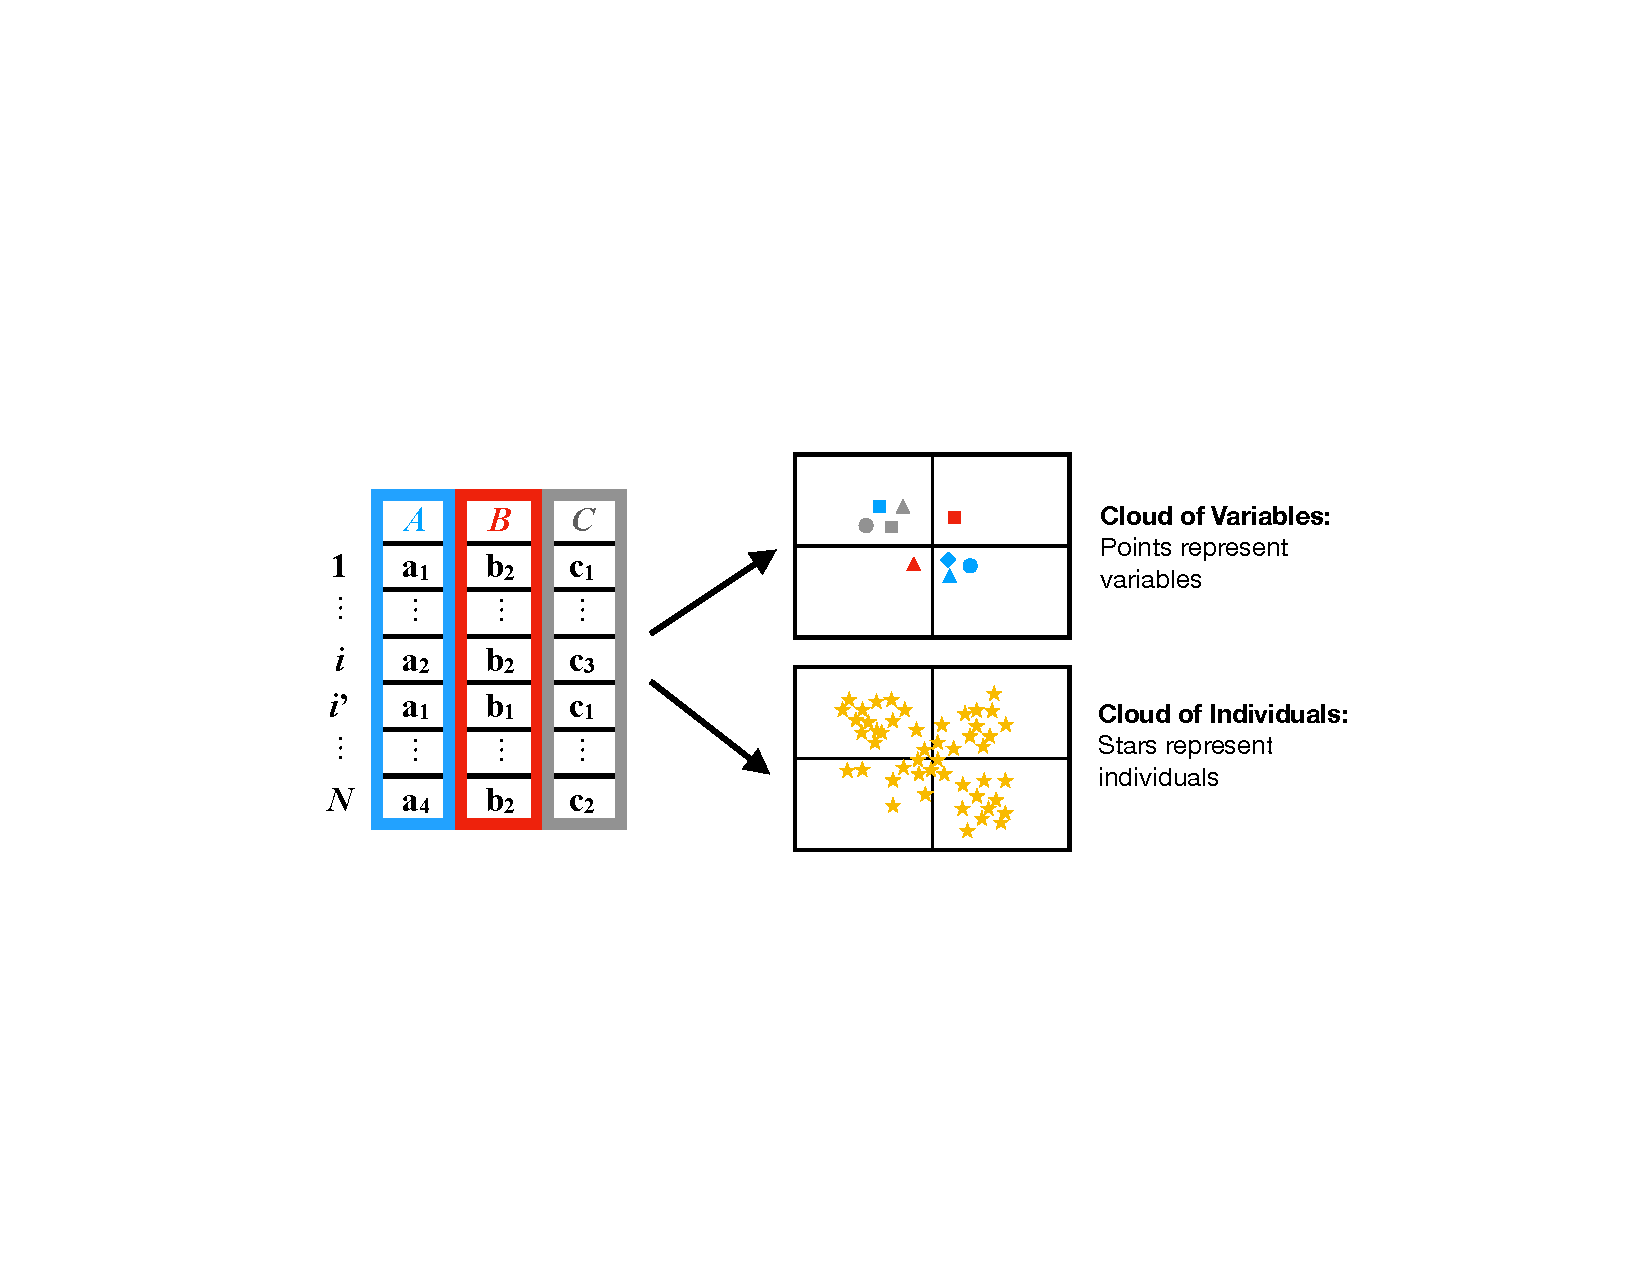
\includegraphics[width=3.4in]{../figs/mcaIdeaNew.pdf}
\caption{Clouds of points generated by MCA}
\label{fig:fig_MCAillustration} 
\end{figure}

The contribution of a category point \(M^k\) to the overall variance is
the ratio of the amount of the variance of the cloud due to category
\(k\). The contribution of a question \(q\) is the sum of the
contributions of its categories. Contributions can be calculated as
shown below:

\begin{equation}
\begin{aligned}[b]
\label{eq:contribMk}
\text{Ctr}_k &= \frac{1-f_k}{K-Q}, \quad \text{Ctr}_q &= \frac{K_q -1 }{K-Q}
\end{aligned}
\end{equation}

The variance of the cloud is simply
\(V_{\text{cloud}} = \frac{K}{Q} - 1\) and the mean of eigenvalues is
given by \(\bar{\lambda} = \frac{1}{Q}.\)

For interpreting an axis, we use the method of contributions of points
and deviations. Due to the high dimensionality of the clouds, the
variance rates of the principal axes are generally low.
\cite{benzecri1992correspondence} proposed to use modified rates in
order to better understand the importance of the first principal
dimensions. Variance rates are calculated following the steps below:

For \(l = 1,2,...,l_{\max}\) such that \(\lambda_l > \bar{\lambda}\)
calculate:

\begin{enumerate}
\def\labelenumi{\arabic{enumi}.}
\item
  the pseudo-eigenvalue
  \(\lambda^\prime = \left( \frac{Q}{Q-1} \right)^2(\lambda_l - \bar{\lambda})^2\),
\item
  the sum \(S=\sum_{l=1}^{l_{\max}} \lambda^{\prime} _l\)
\end{enumerate}

Then for \(l < l_{\max}\) the modified rates are equal to
\(\tau^\prime _l = \lambda^\prime_l / S\)

MCA can be seen as a particular case of weighted principal component
analysis, in which a set of multidimensional points exists in a high-
dimensional space where distance is measured by a weighted Euclidean
metric and the points themselves have differential masses. A lower
dimensional solution is obtained by determining the closest plane to the
points in terms of weighted least-squared distance, and then projecting
the points onto the plane for visualization and interpretation. The
low-dimensional subspace that fits the points as closely as possible can
be obtained compactly and neatly using the generalized singular-value
decomposition (SVD) of the data matrix \cite{greenacre2006multiple}.

\hypertarget{the-health-and-retirement-study-hrs-dataset}{%
\section{The Health and Retirement Study (HRS)
Dataset}\label{the-health-and-retirement-study-hrs-dataset}}

Created in 1990 and launched in 1992 by the National Institute on Aging
(NIA) and Social Security Administration, the Health and Retirement
Study (HRS) surveys collect every two years of data from more than
22,000 Americans over 50 years old. It is the first longitudinal study
of Americans approaching the economic and health aspects in the same
survey and being the largest nationally representative
multi-disciplinary panel study of Americans aged 50 and older. The study
was created and maintained by the Institute for Social Research (ISR)
Survey Research Center (SRC) at the University of Michigan. The
methodology uses an interview typically conducted in person, by
telephone with a duration of approximately 2.72 hours, including topics
such as health status and conditions, employment history, internet
usage, health care utilization, cognitive status, disability status,
physical functioning, housing status, family characteristics, work
environment characteristics, among others.

The HRS data are organized in public and restricted materials and
contains survey records produced by ISR and third parties which publish
data based on processed HRS data. The public HRS files are divided into
three files called HRS Core, Exit, and Post-Exit. Also, the data
produced by the RAND (``Research ANd Development'') Center for the Study
of Aging, and USC Program on Global Aging, Health, and Policy, and data
produced by researchers is available. This study uses the following data
products: HRS Core Cognition Section (D) \cite{sonnega2014health}, HRS
Left-Behind Questionnaires Section LB \cite{smith2013psychosocial}, and
the RAND HRS Longitudinal File 2014 (V2) \cite{HRS2014}. All the data
used in this work was related to the survey waves of 2006, 2008, 2010
and 2012. The Cognition section provides the variables related to memory
performance and subjective memory, not included memory diseases which
are not part of variables used in the studies. The psychosocial and
lifestyle questionnaires from 2006 to 2010 are self-administered
questionnaires that stay with the respondents after the completion of an
in-person core interview, covering six main areas: subjective
well-being, lifestyle and experience of stress, quality of social ties,
personality traits, work-related beliefs, and self-related beliefs.

Data used in this study comes from waves 08, 09, 10 and 11,
corresponding to years 2006, 2008, 2010, and 2012 respectively. The
sociodemographic data was extracted from the RAND datasets with
variables such as gender (male, female), age, race (White/Caucasian,
Black/African American, other), ethnic group (Hispanic, non-Hispanic),
education (none, elementary, middle school, high school, college,
other), and military service (veteran, non-veteran) Information
associated with mental health was separated in data related to
depression and anxiety. Depression variables extracted from the RAND
dataset capture the result of the mental health index derivation using
the CES-D scale (Center for Epidemiological Studies Depression Scale).
The CES-D score is constructed based on the sum of five negative
indicators minus two positive indicators. All the positive and negative
indicators are obtained from a closed-ended question with \emph{yes} or
\emph{no}, as the possible answers \cite{cesd}.

\hypertarget{results-and-discussion}{%
\section{Results and Discussion}\label{results-and-discussion}}

\hypertarget{multiple-correspondence-analysis}{%
\subsection{Multiple Correspondence
Analysis}\label{multiple-correspondence-analysis}}

MCA was performed on a combined dataset from respondents of the 2008 and
2010 waves. Notice that the participants of the 2008 survey are
different than those from the 2010 survey. The clouds patterns for every
wave were examined to confirm that the overall geometric representations
were similar regardless of the number of participants in each wave, or
the year in which the survey responses were collected. Therefore, the
results shown in this study include responses for two different years
with different participants to test the ability of the technique on a
large set of observations (other years combinations were calculated and
very similar results were obtained using the geometric data analysis
framework discussed here). The dimensions of the final dataset used in
this analysis are \(9732 \times 34\), where each row of the tabular data
set represents one of the survey respondents and each column is a
question included in the questionnaire. A summary of the frequency of
responses is shown in Table \ref{tab:fknkTop12}.

\begin{table}[ht!]
\caption{Response frequencies (absolute $n_k$ and relative $f_k$), and contributions ($\text{Ctr}_k$) of  top categories by $\text{Ctr}_k$ and levels} 
\centering
\begin{tabular}{lrrr}
  \hline
  Category & $n_k$ & $f_k$ & $\text{Ctr}_k$ \\ 
  \hline
  sophisticated\_Not at all & 2159 & 0.22 & 0.0093 \\ 
  imaginative\_A lot & 3109 & 0.32 & 0.0081 \\ 
  creative\_A lot & 2668 & 0.27 & 0.0086 \\ 
  caring\_A little & 345 & 0.04 & 0.011 \\ 
  talkactive\_A lot & 2823 & 0.29 & 0.0085 \\ 
  friendly\_A little & 372 & 0.04 & 0.011 \\ 
  careless\_Some & 993 & 0.10 & 0.011 \\ 
  responsible\_Some & 1729 & 0.18 & 0.0098 \\ 
  responsible\_A little & 236 & 0.02 & 0.012 \\ 
  nervous\_Not at all & 3101 & 0.32 & 0.0081 \\ 
  worry\_Not at all & 1625 & 0.17 & 0.0099 \\ 
  moody\_Some & 1470 & 0.15 & 0.01 \\ 
   \hline
\end{tabular}
\label{tab:fknkTop12}
\end{table}

The cloud in Fig. \ref{fig:biplot} is the projection of the full cloud
onto the plane of the principal axes 1 and 2, that is, onto the
principal plane 1-2. The location of the top contributing categories is
also shown, in a graph known as the \emph{biplot} of individuals and
variables. In Fig. \ref{fig:plane34} the projection on plane 3-4 is
presented, and the participants are colored by gender. Notice that in
this plane, a clear separation is found by this categorical variable,
and the collection of associated categories is informative of the
pattern shown by the survey respondents.

\begin{figure}[H] 
\centering 
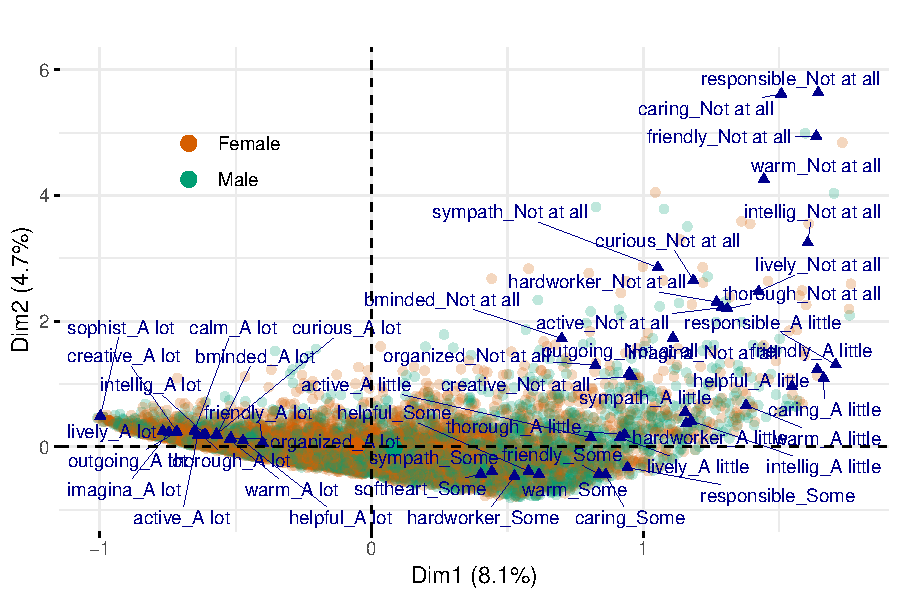
\includegraphics[width=2.93in]{../figs/newbiplot12.pdf}
\caption{Projection onto the first two principal dimensions}
\label{fig:biplot} 
\end{figure}

\begin{figure}[H] 
\centering 
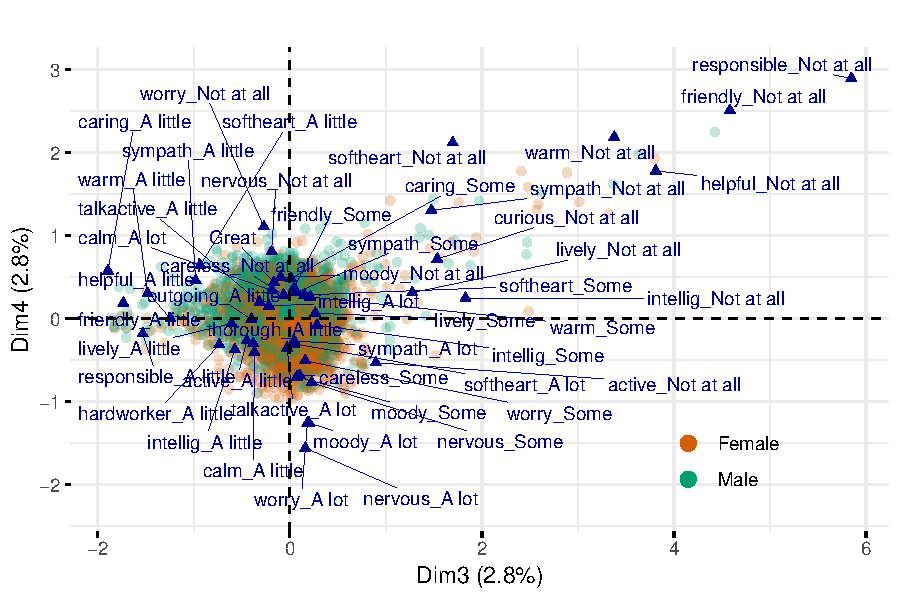
\includegraphics[width=2.93in]{../figs/newbiplot34.pdf}
\caption{Biplot in dimensions 3 and 4 with top contributing variables. Respondents are color-coded based on the supplementary variable gender}
\label{fig:plane34} 
\end{figure}

The coordinates of the first 4 dimensions for the top 12 categories
(sorted by contribution \(\text{Ctr}_k\) and level of agreement) are
shown in Table \ref{tab:top12coord}. Large coordinate measures suggest
that the categories of a variable are better separated along that
dimension, while similar coordinate measures for different variables in
the same dimensions indicate that these variables are related to each
other.

\begin{table}[H]
\caption{Coordinates of the first 4 dimensions for the top 12 categories (sorted by contribution $\text{Ctr}_k$ and level of agreement)} 
\centering
\begin{tabular}{lrrrr}
  \hline
  Variable & Dim 1 & Dim 2 & Dim 3 & Dim 4 \\ 
  \hline
  sophisticated\_Not at all & 0.52 & 0.32 & 0.03 & -0.14 \\ 
  imaginative\_A lot & -0.75 & 0.23 & -0.20 & 0.04 \\ 
  creative\_A lot & -0.72 & 0.25 & -0.23 & 0.03 \\ 
  caring\_A little & 1.66 & 1.09 & -1.90 & 0.58 \\ 
  talkactive\_A lot & -0.53 & 0.22 & -0.03 & -0.35 \\ 
  friendly\_A little & 1.64 & 1.23 & -1.73 & 0.19 \\ 
  careless\_Some & 0.32 & 0.08 & 0.10 & -0.68 \\ 
  responsible\_A little & 1.71 & 1.31 & -1.53 & -0.18 \\ 
  responsible\_Some & 0.94 & -0.33 & 0.07 & -0.06 \\ 
  nervous\_Not at all & -0.31 & 0.22 & -0.19 & 0.81 \\ 
  worry\_Not at all & -0.34 & 0.39 & -0.27 & 1.11 \\ 
  moody\_Some & 0.27 & 0.02 & 0.07 & -0.70 \\ 
   \hline
\end{tabular}
\label{tab:top12coord}
\end{table}

In Table \ref{tab:modRate} the modified rates for the first principal
axes produced by MCA on the HRS survey data are shown.

\begin{table}[!ht]
\caption{Variances of axes, variance and modified rates} 
\centering
\begin{tabular}{rcccccc}
  \hline
  Axes & 1 & 2 & 3 & 4 & 5 & 6\\ 
  \hline
  Eigenvalue ($\lambda_l$) & 0.244 & 0.142 & 0.086 & 0.085 & 0.070 & 0.063\\  
  Variance rate                & 0.081 & 0.047 & 0.029 & 0.028 & 0.023 & 0.021\\  
  Modified rate ($\tau_l$) & 0.688 & 0.180 & 0.039 & 0.038 & 0.019 & 0.012\\ 
  \hline
\end{tabular}
\label{tab:modRate}
\end{table}

Fig. \ref{fig:screeplot} shows the percentages of variance of the first
10 dimensions. The first principal axis explained 8.11\% of the
principal inertia, the second principal axis explained 4.72\%, and none
of the remaining principal axes explained more than 3\%. Using the
modified variance rates \(\tau_l\) one can see that the first two
dimensions explain about 86.8\% of the variance in the data.

\begin{figure}[!ht] 
\centering
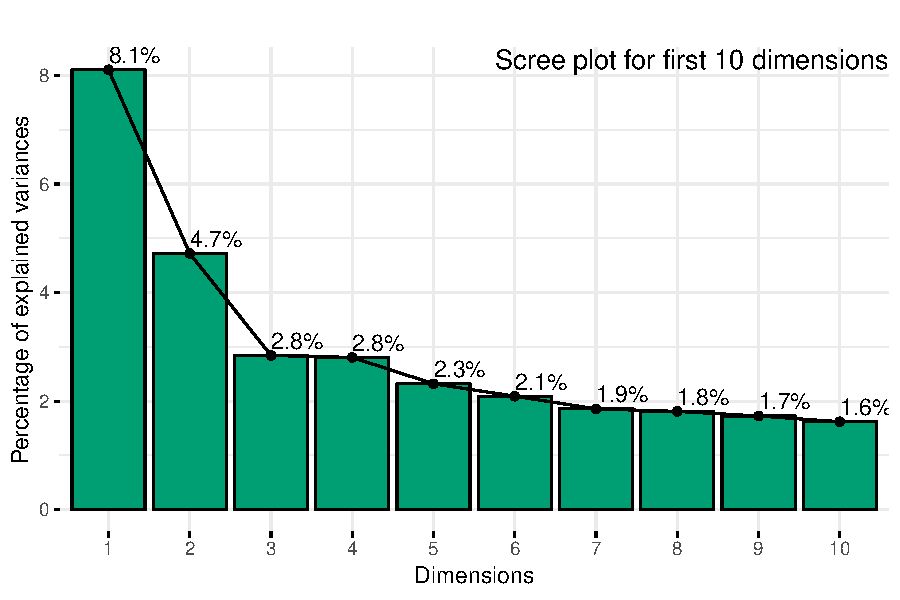
\includegraphics[width=3in]{../figs/screeplot.pdf}
\caption{Variation explained by each principal component}
\label{fig:screeplot} 
\end{figure}

\begin{table}[!ht]
\caption{Squared correlation between each variable and the principal dimension} 
\centering
\begin{tabular}{rrrrr}
  \hline
 & Dim 1 & Dim 2 & Dim 3 & Dim 4 \\ 
  \hline
 level\_of\_education & 0.03 & 0.02 & 0.01 & 0.08 \\ 
  subjective\_memory & 0.10 & 0.04 & 0.01 & 0.07 \\ 
  sophisticated & 0.21 & 0.07 & 0.03 & 0.01 \\ 
  broadminded & 0.25 & 0.18 & 0.08 & 0.01 \\ 
  curious & 0.28 & 0.19 & 0.09 & 0.01 \\ 
  intelligent & 0.37 & 0.21 & 0.13 & 0.03 \\ 
  imaginative & 0.33 & 0.14 & 0.06 & 0.01 \\ 
  creative & 0.28 & 0.15 & 0.05 & 0.01 \\ 
  sympathetic & 0.27 & 0.19 & 0.10 & 0.11 \\ 
  softhearted & 0.22 & 0.15 & 0.12 & 0.17 \\ 
  caring & 0.36 & 0.21 & 0.26 & 0.14 \\ 
  warm & 0.44 & 0.22 & 0.25 & 0.09 \\ 
  helpful & 0.39 & 0.18 & 0.16 & 0.04 \\ 
  talkactive & 0.17 & 0.06 & 0.04 & 0.07 \\ 
  active & 0.35 & 0.22 & 0.09 & 0.02 \\ 
  lively & 0.42 & 0.23 & 0.14 & 0.01 \\ 
  friendly & 0.40 & 0.21 & 0.20 & 0.08 \\ 
  outgoing & 0.33 & 0.14 & 0.06 & 0.02 \\ 
  careless & 0.06 & 0.07 & 0.00 & 0.10 \\ 
  thorough & 0.33 & 0.18 & 0.07 & 0.02 \\ 
  hardworker & 0.31 & 0.20 & 0.08 & 0.01 \\ 
  responsible & 0.30 & 0.18 & 0.19 & 0.03 \\ 
  organized & 0.21 & 0.13 & 0.05 & 0.02 \\ 
  calm & 0.27 & 0.17 & 0.08 & 0.08 \\ 
  nervous & 0.05 & 0.09 & 0.02 & 0.47 \\ 
  worry & 0.04 & 0.09 & 0.02 & 0.46 \\ 
  moody & 0.07 & 0.07 & 0.01 & 0.22 \\ 
   \hline
\end{tabular}
\label{tab:varsCorrelation}
\end{table}

In Table \ref{tab:varsCorrelation} the squared correlation between each
of the questions in the survey considered in this study and the
principal dimensions is shown.

\hypertarget{clustering}{%
\subsection{Clustering}\label{clustering}}

Geometric data analysis methods have the potential to be used as a
pre-processing step for clustering, given the representation in a lower
dimensional space provided by the principal component technique of
choice \cite{jolliffe2002principal}. In this work, a hierarchical
clustering algorithm is performed using the coordinates of each
respondent in the lower dimensional space generated by the MCA
procedure. Hierarchical clustering requires to define a distance and an
agglomeration criterion \cite{tan2013data}. Here the traditional
Euclidean distance for calculating dissimilarities between observations
and the complete linkage agglomeration method were used
\cite{ding2002cluster}.

\begin{figure}[!ht] 
\centering 
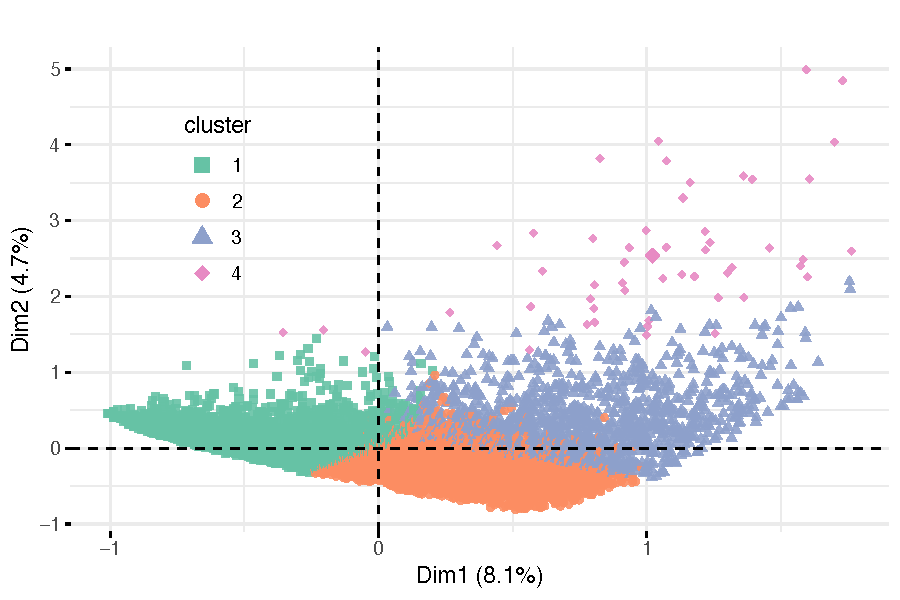
\includegraphics[width=3.2in]{../figs/new_hclust.pdf}
\caption{Hierarchical clustering using principal dimensions generated by multiple correspondence analysis.}
\label{fig:hclust} 
\end{figure}

\begin{figure*}[!ht] 
\centering 
\subfloat[]{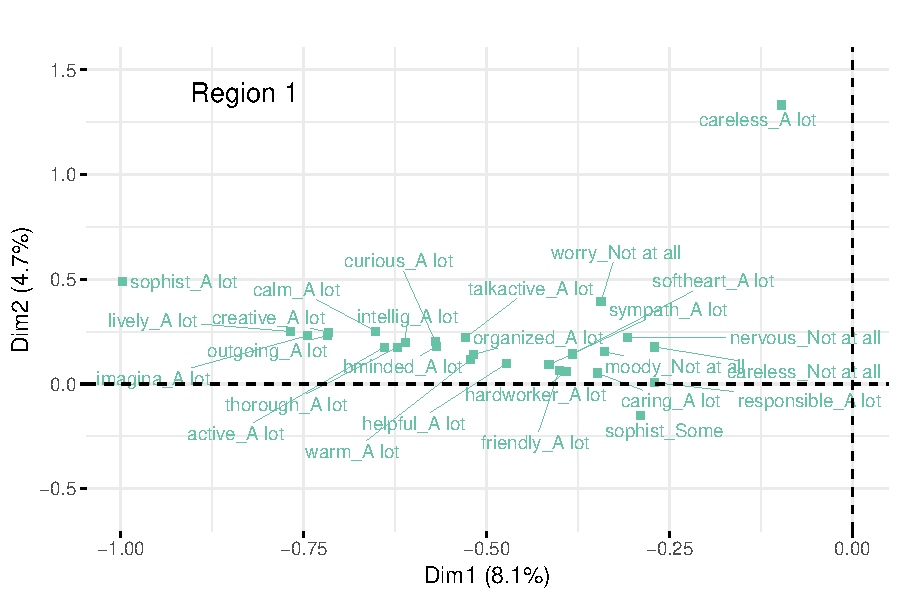
\includegraphics[width=3.5in]{../figs/region_1_plot.pdf}%
\label{fig_first_case}}
\hfil 
\subfloat[]{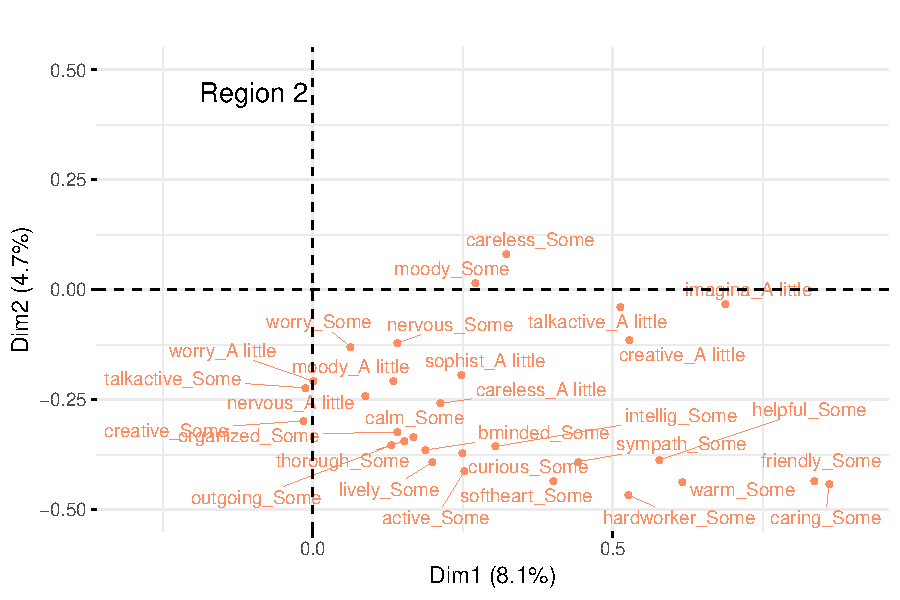
\includegraphics[width=3.5in]{../figs/region_2_plot.pdf}% 
\label{fig_second_case}} 
\hfil 
\subfloat[]{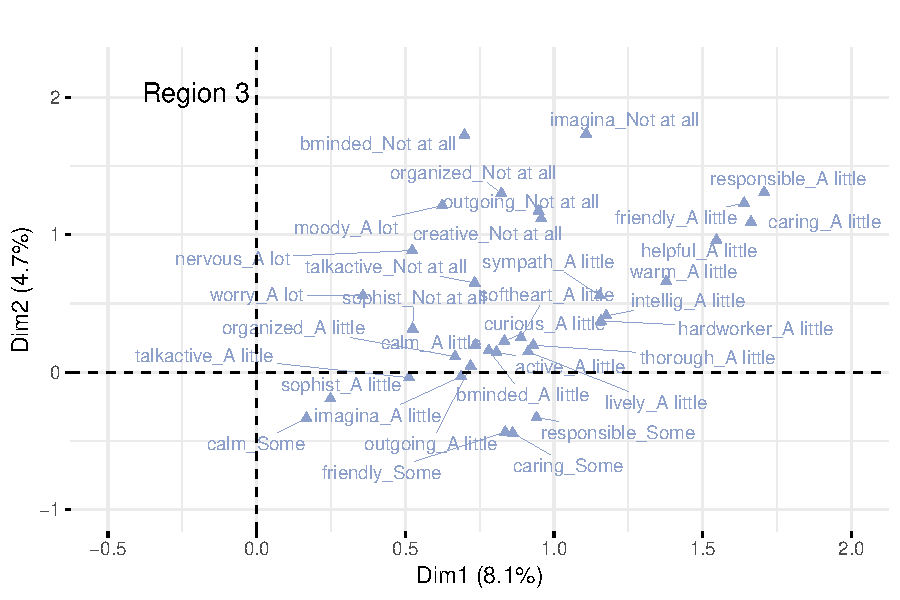
\includegraphics[width=3.5in]{../figs/region_3_plot.pdf}%
\label{fig_third_case}}
\hfil
\subfloat[]{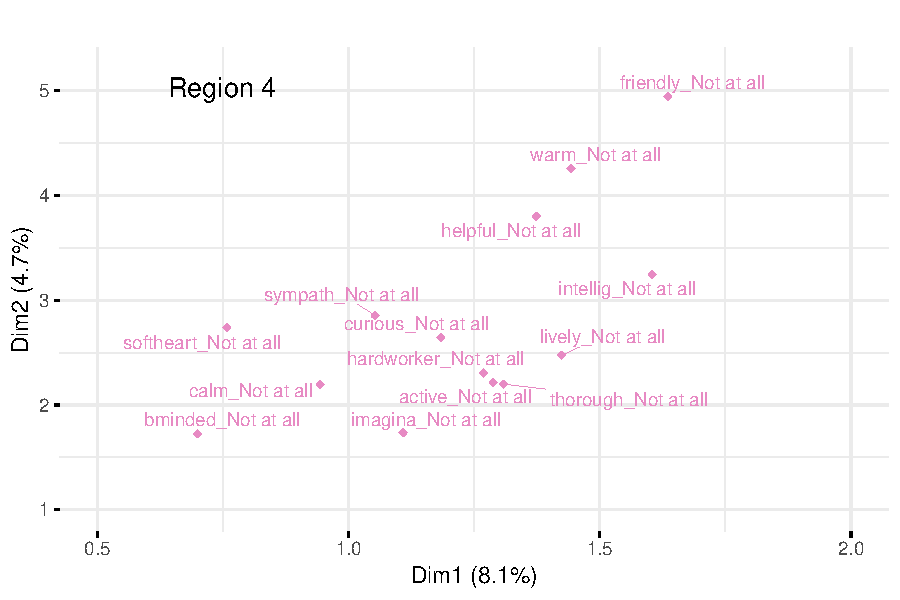
\includegraphics[width=3.5in]{../figs/region_4_plot.pdf}% 
\label{fig_fourth_case}} 
\caption{Clouds of categories: (a) Region 1, (b) Region 2, (c) Region 3, (d) Region 4} 
\label{fig:regions12Clust} 
\end{figure*}

% \begin{figure}[h!]
% \centering
%   \subfloat[]{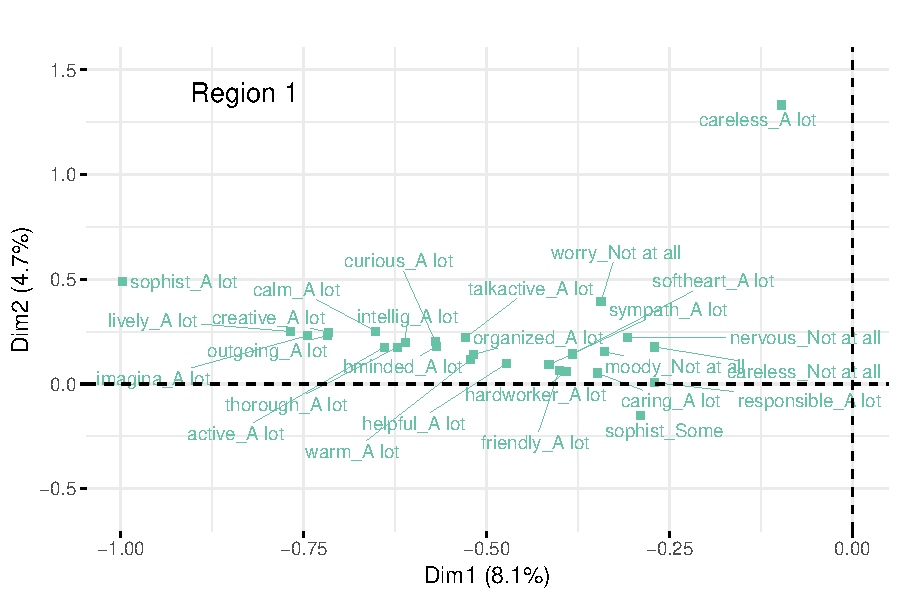
\includegraphics[width=3.5in]{../figs/region_1_plot.pdf}}
%   \subfloat[] {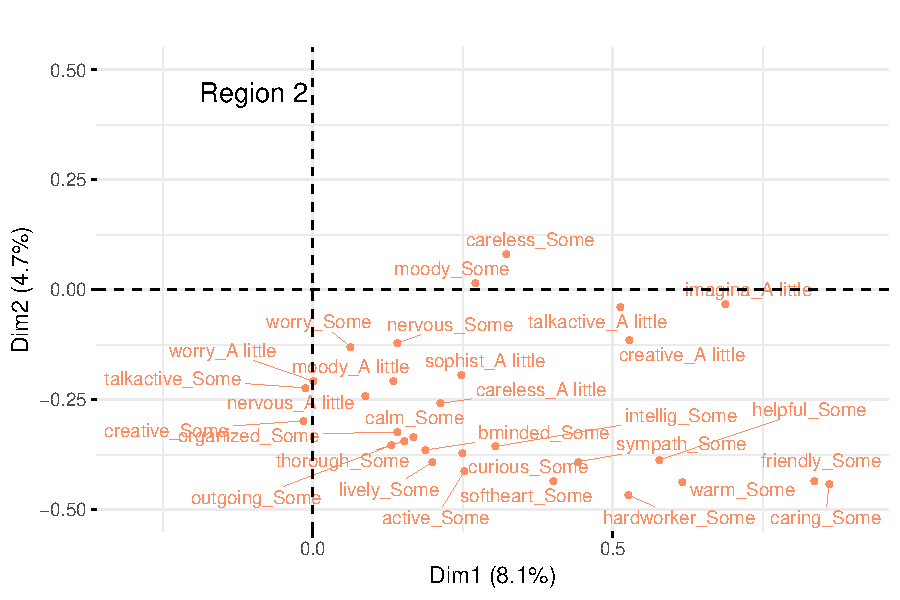
\includegraphics[width=3.5in]{../figs/region_2_plot.pdf}}\hfill
%   \subfloat[]{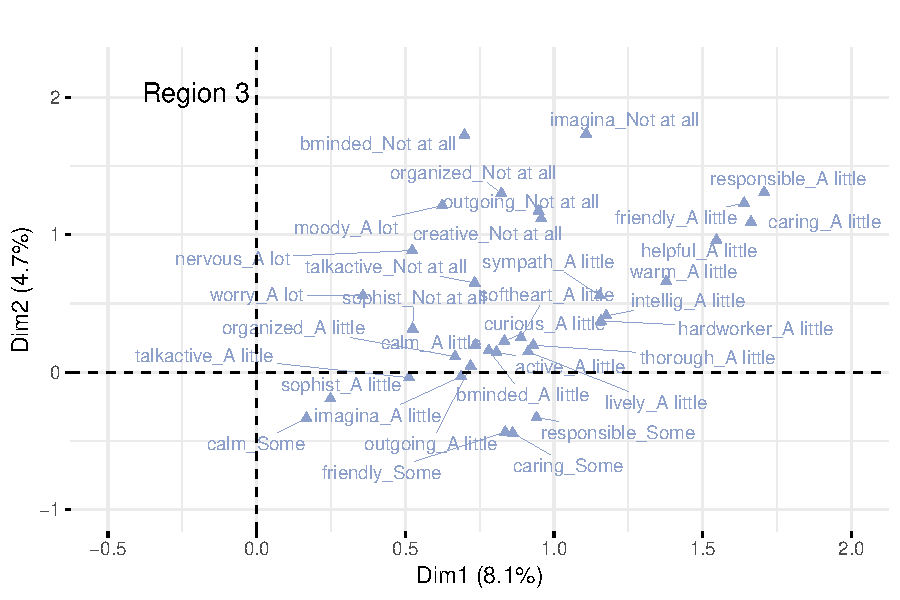
\includegraphics[width=3.5in]{../figs/region_3_plot.pdf}}
%   \subfloat[]{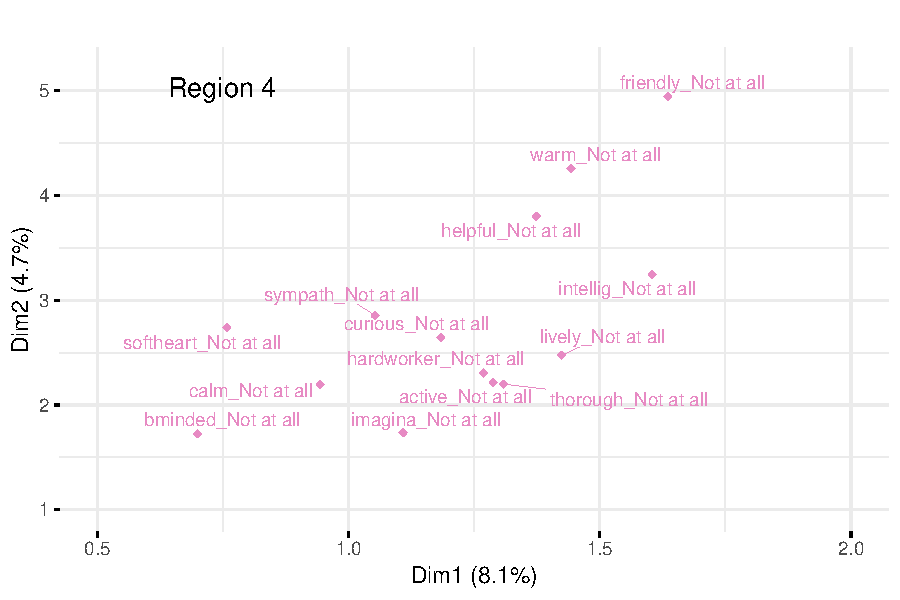
\includegraphics[width=3.5in]{../figs/region_4_plot.pdf}}\hfill
% \caption{XXXXXXX: (a) Region 1, (b) Region 2, (c) Region 3, (d) Region 4} 
% \label{fig:1}
% \end{figure}







The findings of this hierarchical clustering confirm a natural grouping
for the participants of the survey: the tendency of survey respondent to
use the levels of agreement with the different questions that are part
of the questionnaire, namely, \emph{``a lot''}, \emph{``not at all''},
\emph{``some''} and \emph{``a little''}. These levels of agreements are
well separated in distinct regions within the plane of the first 2
principal dimensions. Fig. \ref{fig:regions12Clust} shows the categories
that fall in the regions suggested by the clustering procedure results
shown in Fig. \ref{fig:hclust}.

Variables indicating gender, veteran status, ethnicity, race, and
depression status were used as supplementary categories. A supplementary
category (sometimes called illustrative category), is a category that is
not used to define the distance between individuals. Recall that every
variable has multiple levels related to the rate of agreement with the
associated question. Table \ref{tab:supplCoord} shows the coordinates in
the first four dimensions for the supplementary variables considered
here. The deviation between female and male respondents on axis 4 is
notable (\(\vert -0.183 - 0.277 \vert = 0.46\)) confirming the suggested
grouping observed in Fig. \ref{fig:plane34} for plane 3-4.

\begin{table}[ht]
\caption{Coordinates of the supplementary variables on the first four axes} 
\centering
\begin{tabular}{rlrrrr}
  \hline
  Category & Dim 1 & Dim 2 & Dim 3 & Dim 4 \\ 
  \hline
  \hline
  Female & -0.11 & 0.04 & 0.06 & -0.18 \\ 
  Male & 0.17 & -0.05 & -0.09 & 0.28 \\ 
  \hline
  non-veteran & -0.05 & 0.03 & 0.03 & -0.09 \\ 
  veteran & 0.17 & -0.10 & -0.09 & 0.32 \\ 
  \hline
  hispanic & 0.18 & 0.19 & 0.20 & -0.21 \\ 
  non-hispanic & -0.01 & -0.02 & -0.02 & 0.02 \\ 
  \hline
  black & -0.06 & 0.34 & -0.05 & 0.08 \\ 
  other & 0.00 & 0.18 & 0.03 & -0.10 \\ 
  white & 0.01 & -0.05 & 0.00 & -0.00 \\ 
  \hline
  Depressed No & -0.05 & -0.05 & -0.01 & 0.09 \\ 
  Depressed Yes & 0.43 & 0.45 & 0.11 & -0.73 \\ 
   \hline
\end{tabular}
\label{tab:supplCoord}
\end{table}

The four regions identified here, and shown in Fig.
\ref{fig:regions12Clust}, express consistency category levels of the
variables related to the personality scale \cite{lachman1997midlife}
supplied by the HRS Core LB dataset. The personality scale used in this
work covers five aspects: conscientiousness, neuroticism, extroversion,
agreeableness, and openness. The individuals present in Region 1 have an
open personality and actively seek for new experiences, while
individuals in Region 3 and 4 do not exhibit this characteristic,
holding all the low levels of this perception which is defined by a
\emph{``Not at all''} response in most cases. Similarly, the aspect of
conscientiousness (which is related to organization, persistence,
control, and motion in goal) is a substantial characteristic for
individuals in Region 1, and its weakest trace is found in individuals
located in Regions 3 and 4. In general, Region 2 holds individuals which
scale all the four main characteristics as \emph{``Some''} and \emph{``A
little''} levels, with a high frequency of extraversion and neuroticism,
that combined depict the \emph{``style of well-being''} described in the
sample report in \cite{costa_nodate}. Individuals with low levels of
neuroticism and extraversion (N-E-Low-keyed) maintain considerable
indifference towards good or bad news, sometimes impacting their
interpersonal relationships. In contrast to Region 3, which holds the
extreme lower levels like \emph{``A little''} and \emph{``Not at all''}.
Region 2 is the middle point for all the ``Big 5'' personality
characteristics collected in the HRS Core LB survey.

In this work, the R packages \texttt{dplyr} \cite{Refdplyr} and
\texttt{ggplot2} \cite{ggplotBook} were used for data wrangling and
visualization, and the \texttt{haven} package \cite{wickham2018haven}
for importing data. The MCA algorithm used in this study corresponds to
the implementation of the algorithm available in the \texttt{FactoMineR}
package \cite{le2008factominer}, that includes a collection of methods
for multivariate data analysis. Additionally, the \texttt{factoextra} R
package was used for visualization and interpretation \cite{factoextra}.

\hypertarget{conclusions}{%
\section{Conclusions}\label{conclusions}}

The use of unsupervised techniques presented in this work represents an
opportunity to extract valuable insights from longitudinal datasets like
the one made available by the US Health and Retirement Study. MCA allows
for new interpretations and discovery of patterns that take advantage of
the qualitative nature of the data collected from survey respondents.
The hierarchical clustering technique applied to the low dimensional
representation of participants, provided by the MCA method, suggested a
reasonable separation of the respondent profile as characterized by a
personality scale. Results provided by this approach may be used to
explore other areas that have yet to be captured using the items in the
questionnaires, helping in the design of the survey and sampling
procedure, and allowing for correlation studies with other physical and
mental health indicators.

\hypertarget{acknowledgment}{%
\section*{Acknowledgment}\label{acknowledgment}}

The HRS (Health and Retirement Study) is sponsored by the National
Institute on Aging (grant number NIA U01AG009740) and is conducted by
the University of Michigan. The HRS has been approved by the
Institutional Review Board at the University of Michigan. The HRS
obtains informed verbal consent from voluntary participants and follows
strict procedures to protect study participants from disclosure
(including maintaining a Federal Certificate of Confidentiality). The
public data, made available to registered researchers and used in this
study, is de-identified. The authors gratefully acknowledge the support
of Florida Polytechnic University, and would like to thank the anonymous
reviewers for their constructive comments.

\bibliography{mybibfile.bib}

\bibliographystyle{IEEEtran}

\end{document}


